%!TEX root = main.tex

\section{Introduction} % (fold)
\label{sec:introduction}

Many modern software systems consist of a large number of agents that cooperate and compete \cite{}
to achieve \emph{local} and \emph{global} goals. Local goals are specific of single agents
while the global ones refer to the expected emerging behaviour resulting from the interaction of many agents. 
Agents are often located in an environment that can impact on their \emph{goals}.  
For this reason it is crucial to have mechanisms that allow each agent to adapt its behaviour to
the changing environmental conditions while guaranteeing goals achievement. When a change in the environment is perceived, each agent has to use its knowledge to perform specific actions and \emph{adapt} its behaviour.
Unfortunately, only in rare cases agents have a complete view of the context where they are operating;  often only a partial view is available.  It is then important to develop tools to be used 
to support dynamic adaptation of agents also in presence of partial information about the operating environment.

\paragraph{Adaptive systems} % (fold)
\label{par:adaptive_systems}
The issue of programming adaptive agents is present in many scenarios. Typically, each adaptive agent 
%knows its own features but it 
does not have complete information of the activities taking place in the surrounding environment. 
Thus, 
%Since it has a partial knowledge of the environment, 
methodologies are needed to take decisions to adapt to circumstances. The information about the state of the environment are usually stored in a set of \emph{control data} that are used for \emph{adaptation}. A system is said to be adaptive when its behaviour and its run-time decisions depend directly upon this set of \emph{control data}~\cite{BruniCGLV12}.

Examples of adaptive systems involve agents like robots that have to navigate towards a light source, gather resources, rescue victims while avoiding to fall into traps or to interfere with each other.
% Examples of adaptive systems are swarms of robots, coordinating to reach specific goal like navigating towards a light source, gathering resources, rescuing victims, \ldots \  while avoiding traps or collisions between components of the swarm.
Another example  can be found in cloud computing scenarios where physical machines have to adapt in order to guarantee availability of specific virtual ones while guaranteeing availability and quality of service parameters agreed with the clients. 
% A third example of adaptive systems are electrical car fleets that by exploiting exchange of messages whenever possible have to optimize at run time the transport of people, the use of parking lots or of charging stations while taking into account traffic situation and timing constraints.
%
% agent/environment approach
%In these scenarios, components interact with the other entities in the environment in which they are operating but have only a limited knowledge of the environment itself and of the status of other components.
% paragraph adaptive_systems (end)

\paragraph{Methodology} % (fold)
\label{par:methodology}
% general approach
In this paper, we propose a general methodology to be used when dealing with adaptive agents that interacts with an external environment by executing actions and perceiving signals. The environment is formed by all the components that are external to the agent; the controller of each agent exploits the observable history (sequences of actions and observations) to decide the action to perform in order to achieve the specific target in an optimal way. The target is formally specified at design-time by means of a temporal logic formula  that expresses properties of observation sequences in probabilistic and partially observable domains. A methodology is introduced to resolve agents' choices by relying on model checking~\cite{Katoen-Baier};  the action to be performed are determined by taking into account the path that maximizes the probability of satisfying the provided target formula.

We consider systems whose behaviour is fully described but such that their current state is 
%not directly (partially) 
only partially observable. Agents are described by means of  nondeterministic models and the environment with probabilistic ones. By composing these two systems we obtain a partially observable process in which every state is split in two parts: the controller, that is fully observable, and the environment, that is not directly observable. The history of performed actions and perceived observations is used to refine a probabilistic belief about the current state.

The classical model checking algorithm is ``adapted'' to partially observable models in order to check the probabilities to satisfy the temporal logic formula that describes the goal. The partially observable model is transformed into a fully observable one, observations are used to label states and the measure of satisfiability of a property is reduced to the one in a fully observable context. The adaptation strategy consists then in choosing the action that maximize the chances to satisfy the goal formula. Depending on the needs, it might be appropriate to minimize the risk or to maximize the opportunities. %Synthesizing these kind of strategies intrinsically ensure a correct behaviour with respect to the chosen goal formula.

% runtime
Since the (storage and computing)  resources available to the agents are often limited, the model checking approach may look expensive. But, it has to be considered that, we rely on a two steps  algorithm; the first step has an exponential complexity while the second one is polynomial.  The former one is computed just once and only the latter
%, that is the interaction with the environment, 
has to be computed at run-time. 

% paragraph methodology (end)

\paragraph{A running example} % (fold)
\label{par:a_running_example}

\setlength\intextsep{0pt}
\begin{wrapfigure}[15]{r}{0.3\textwidth}	
%\vspace{-1cm}
%\begin{figure}[htb]
	\begin{center}
	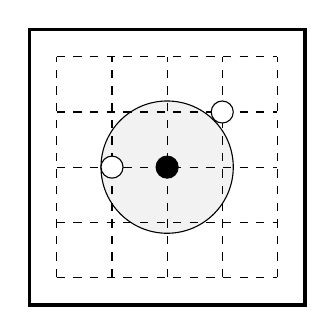
\begin{tikzpicture}[scale=.7]
	\begin{scope}
%	  \filldraw [fill=gray!10] (4,4) circle (1.4); % raggio esteso
	  \filldraw [fill=gray!10] (3,3) circle (1.2); % raggio ridotto
	
	  \draw[dashed] (1, 1) grid (5, 5);
	  \draw[very thick, scale=1] (0.5, 0.5) rectangle (5.5, 5.5);
	
	  \filldraw [fill=black!100] (3,3) circle (0.2);
		
	  \filldraw [fill=white!50] (4,4) circle (0.2);
	  \filldraw [fill=white!50] (2,3) circle (0.2);
%	  \filldraw [fill=white!50] (2,2) circle (0.2);
	\end{scope}
	\end{tikzpicture}
	\end{center}
	\caption{Bird's-eye view representation of the robot arena scenario}
	\label{fig:arenarobot}
%\end{figure}
%\vspace{-.71cm}
\end{wrapfigure}

In the paper we will use a simple robotic scenario as a running example. We consider a robot that moves inside an arena with other robots. %has to reach a destination avoiding other robots or obstacles. 
The proximity sensors of the robot analyse the surrounding area to locate obstacles and their positions; the acquired information is then used by the robot to determine the direction to take.

Figure~\ref{fig:arenarobot} provides a pictorial rendering of the scenario; the arena is represented as a $5\times 5$ grid and is bounded by four walls. The dashed grid represents the agents' walkable paths. %the paths walkable by agents.
We assume that at any step a robot can move from a cross to an adjacent one.
The arena contains four agents; the main robot, the black one, and three white robots that, it is assumed, follow a random trajectory. The main robot monitors the five local positions (north, south, east, west and the central position) via proximity sensors. It is able to perceive other agents within a range of visibility represented by a gray circle; in the figure, it can perceive just one agent at west.

In this kind of setting we may want to attribute different goals to the black robot, like collision-avoidance or tracking the white robots' movement. We use this simple scenario to show how goals can be formally represented and, starting from them, how good the results obtained by the synthesis of an adaptive controller are.
%are the results obtained by the synthesis of an adaptive controller.

% example application
%Let's consider the case in which the robot has to reach a given target position minimizing the number of collisions with other robots or obstacles, we can imagine a system composed by the main agent (the robot) running in parallel with the environment. The environment will be composed by the other robots and by the obstacles that the adaptive robot is able to recognize. When the choice to be taken is related to the direction to follow, the model checker will be used to calculate the probabilities, for each possible local decision, of not colliding with other robots within a certain number of steps. In this way the success probability for each available choice can be determined and then the robot knows that the action to be executed is the one with the highest associated probability.

% paragraph a_running_example (end)

%\paragraph{Literature review} % (fold)
%\label{par:literature_review}
%
%% adaptive systems formalization
%%This work focuses on a formal technique to model several features of an adaptive system. To do that we take inspiration from \cite{Bruni2013} and we model agents' behaviours with transition systems composed together into the global system's behaviour. The most important distinction we make is the one between the adaptive agent and the surrounding environment: the former can be controlled by external actions while the latter may be the result of a further composition among many behaviours of other components.
%%
%%% CSP
%%Communication between adaptive agent and environment works as synchronisation between processes in CSP \cite{BrookesHR84,DengGHM08}, indeed all the components of the system are modeled as parallel processes communicating with each other.
%%The agent's behaviour consists in sending messages to the environment that is always ready to accept incoming requests. This assumption makes the action execution non-blocking for the agent. Moreover, the environment may react in different ways depending on the received message. We have then a two side communication between the adaptive agent and the environment, that is in turn the result of the parallel composition of the behaviour of every external component.
%%\\
%
%% partially observable models
%Partially observable models like \acp{HMM} \cite{Rabiner90} and \acp{POMDP}~\cite{cassandra1998survey} have been successfully employed in many fields like speech-recognition~\cite{Rabiner90} and activity recognition for ambient assisted living~\cite{vicario2015continuous}.
%These models cope with the lack of information typical of an adaptive system. In particular \acp{POMDP} give the possibility to model the partial knowledge in presence of input and output interactions, as sensing and acting procedures. Finding the optimal scheduler is a problem that has been approached in different ways~\cite{LittmanCK95} since many theoretical limits have been proven to subsist: building the optimal scheduler function is PSPACE-complete in case of finite horizon~\cite{Papadimitriou1987} and determining its existence is undecidable for infinite horizon~\cite{MadaniHC99}.
%
%% model checking on partially observable models
%Model checking on \acp{HMM} is proposed in~\cite{ZhangHJ05} together with the extended definitions of branching-time and linear-time logics to include belief states and observation specifications. In this work we adopt a different perspective and we consider observations as label of states. We use classic \ac{LTL} formulae~\cite{Pnueli77} to express properties with probabilistic observations on \acp{POMDP}. 
%
%We want to employ model checking techniques to solve a planning problem, this kind of approach has already been proposed in a similar way in~\cite{Bertoli2001,LagoPT02}. In~\cite{Bertoli2001} the model checking techniques are employed to solve a planning problem, we further exploit the classical algorithm to solve the same problem at run-time. Also the logic used to formulate agent's objectives differs from the goal language proposed in~\cite{LagoPT02} since we focus on the explicit use of observation signals.
%
%%Linear-time model checking on \acp{POMDP} is just one step toward our aim, that is building a scheduler given an \ac{LTL} formula that describe the objective of the adaptive agent. Indeed, given a formula and the formal model of the system we can reuse the \ac{LTL} model checking algorithm to automatize the computation of a scheduler that can control the adaptive agent.
%
%% paragraph literature_review (end)

\paragraph{Structure of the paper} % (fold)
\label{par:structure_of_the_paper}
The rest of the paper is organized as follows. We start by introducing the basic structures and languages that we have chosen
%with preliminaries models, \acp{DTMC}, \acp{MDP} and \acp{POMDP} that are the chosen structures 
to represent agents' behaviour and environment; then we extend them to model the adaptation problem and  
%comprehensive of a \ac{LTL} 
to express goals. Subsequently, we prove correctness of the proposed transformations, present the adaptation algorithm, split into an off-line and on-line phase, and discuss its complexity. Finally, we show some results of the proposed method applied to the robotics example.
% and to a cloud computing scenario.

% paragraph structure_of_the_paper (end)

% section introduction (end)
